\begin{figure}[H]
\centering
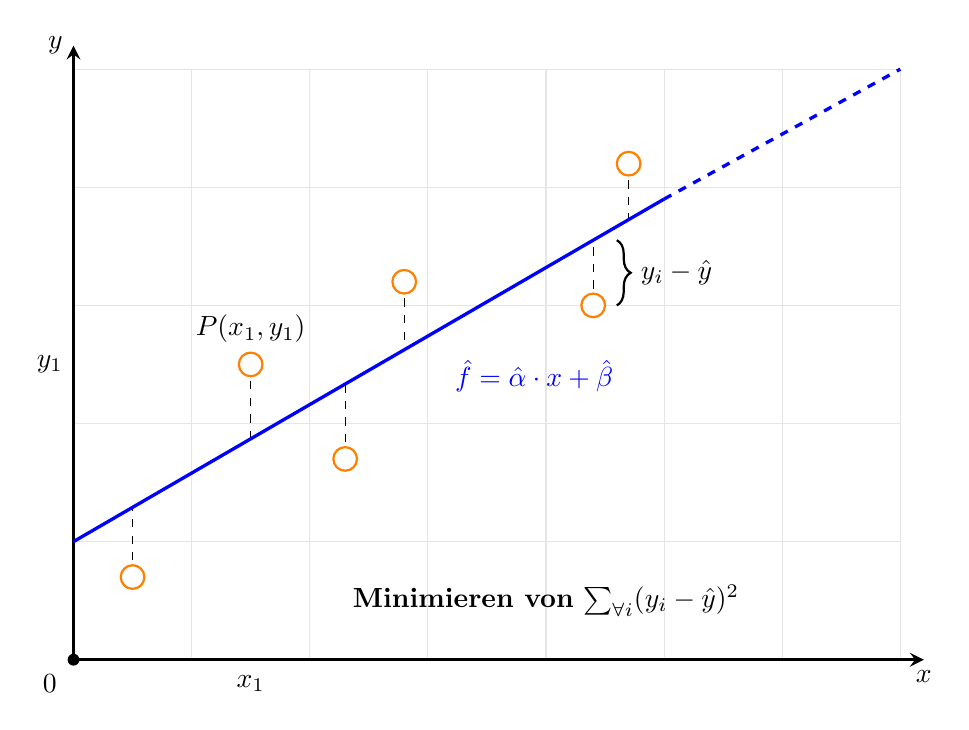
\begin{tikzpicture}[
	scale=1.5,
	axis/.style={
		-stealth,
		very thick
	},
	f/.style={
		very thick,
		blue
	}
]

% Gitter
\draw[gray!20] (0,0) grid (7,5);

% Achsen
\draw[axis] (0,0) -- (7.2,0) node[below]{$\boldsymbol{x}$};
\draw[axis] (0,0) -- (0,5.2) node[left]{$\boldsymbol{y}$};
\fill[black] (0,0) circle[radius=0.05];
\node at(-0.2,-0.2){$\boldsymbol{0}$};

% Punkte
\foreach \x/\y in {0.5/0.7,1.5/2.5,2.3/1.7,2.8/3.2,4.4/3,4.7/4.2}{
	\draw[dashed,domain=\x:\x,variable=\z] (\x,\y) -- plot ({\z},{2.9/5*\z+1});
	\draw[orange,thick,fill=white] (\x,\y) circle[radius=0.1cm];
}

% Funktion
\draw[f] (0,1) -- (5,3.9);
\node[blue] at(3.9,2.4){$\boldsymbol{\hat{f} = \hat{\alpha} \cdot x + \hat{\beta}}$};
\draw[f,dashed] (5,3.9) -- (7,5);

% Geschweifte Klammer
\draw[
	thick,
	black,
	decorate,
	decoration = {
		brace,
		amplitude = 5pt
	}
] (4.6,3.552) -- (4.6,3)
	node[
		midway,
		right,
		xshift = 5pt
] {$\boldsymbol{y_i -  \hat{y}}$};


\node at(-0.2,2.5){$y_1$};
\node at(1.5,-0.2){$x_1$};
\node at(1.5,2.8){$\boldsymbol{P(x_1,y_1)}$};
\node at(4.0,0.5){\textbf{Minimieren von} $\boldsymbol{\sum_{\forall i}(y_i - \hat{y})^2}$};

\end{tikzpicture}
\caption[Graphische Darstellung der linearen Regression]{Graphische Darstellung der linearen Regression\protect\footnotemark}
\label{lr}
\end{figure}
\footnotetext{Abbildung in Anlehnung an \textit{Backhaus} et al., Multivariate Analysemethoden, 2016, S. 71.}